\documentclass{article}
\usepackage{graphicx}
\usepackage{listings}
\usepackage{xcolor}

\begin{document}

\lstdefinelanguage{RISC-V}{
  morekeywords=[1]{
    add, addi, and, andi, auipc, beq, bge, bgeu, blt, bltu, bne, jal, jalr, lb, lbu, lh, lhu, lui, lw, or, ori, sb, sh, sll, slli, slt, slti, sltiu, sltu, sra, srai, srl, srli, sub, sw, xor, xori
  },
  morekeywords=[2]{
    .align, .ascii, .asciiz, .byte, .data, .double, .extern, .float, .global, .half, .space, .text, .word
  },
  sensitive=true,
  morecomment=[l]{\#},
  morestring=[b]",
  morestring=[b]',
}

\definecolor{lightgreen}{RGB}{230, 255, 230}

\lstdefinestyle{mystyle}{
    backgroundcolor=\color{lightgreen},
    basicstyle=\ttfamily\small,
    keywordstyle=\bfseries\color{blue},
    commentstyle=\itshape\color{gray},
    stringstyle=\color{orange},
    numbers=left,
    numbersep=5pt,
    numberstyle=\tiny\color{gray},
    breaklines=true,
    showstringspaces=false,
    tabsize=4
}

\lstset{style=mystyle}


\begin{center}
    {
\includegraphics[width=10cm]{LOGOHABIB.png} \\
    \vspace{10mm}}
    {\Large CE/CS 321/330 Computer Architecture} \\
    \vspace{20mm}
    {\huge \textbf{Final Lab Project}} \\
    \vspace{5mm}
    {\Large \textbf{5-Stage Pipelined Processor To Execute A Single Array Sorting Algorithm}} \\
    \vspace{25mm}
    {\Large \textbf{Group Members}} \\
    \vspace{5mm}
    {\Large Hammad Sajid (hs07606)} \\
    \vspace{5mm}
    {\Large Muhammad Azeem Haider (mh06858)} \\
    \vspace{10mm}
\end{center}

\tableofcontents
\newpage

\section{Sorting Algorithm on a Single Cycle Processor}
\subsection{Selection Sort Assembly Code} 
\begin{lstlisting}[caption={Selection Sort Assembly code}, captionpos=b, language=RISC-V]
addi x11, x0, 6 #an arbitrary value to append in array
addi x29, x0, 6 #initializing size of the array to be 6
addi x30, x0, 0 #initializing offset to store values in array after one another
addi x31, x0, 0 #initializing i = 0 to loop through array to enter values.
addi x28, x0, 6 #temporary reg for checking length

#The code below is to intialize random values in the array
Array:

    sw x11, 0x100(x30)  #store values in array
    addi x31, x31, 1 #performs i = i + 1
    addi x30, x30, 4 #offset + 4 to jump to next memory address to store value
    addi x11, x11, -1 #subtracting 1 to add next value in array (6->5->4....)
    beq x28, x31, filled #if i = size of array, stop.
    beq x0, x0, Array
    
filled:

#After the above code, the array is [6,5,4,3,2,1]

addi x30, x0, 0 #i = 0 (for i loop)
addi x31, x30, 0 #j = 0
addi x29, x0, 0 #for offset calculation
addi x11, x0, 6 #condition to check if i = size of array 

#Code below is for 1st i loop

I_Loop:

    beq x11, x30, Sorted #if i = size of array, array has been sorted
    add x10, x29, x0  #assigning min_index = i
    addi x31, x30, 1 #j = j + 1
    addi x28, x29, 4 #jump to next address

#Code below is for nested j loop
J_Loop:

    beq x31, x11, Swap
    lw x15, 0x100(x28) #load Array[j]
    lw x16, 0x100(x10) #load Array[min_index]
    blt x15, x16, If  #if Array[j] < Array[min_index]
    
    #The code below it to iterate through the jth loop
    
    return: 
    
    addi x31, x31, 1 #perform j = j + 1
    addi x28, x28, 4 #jump to next address
    beq x0, x0, J_Loop #jump to nested j loop
    
    #The code below is to iterate through ith loop.
    
    jump_back:
    
    addi x30, x30, 1 #perform i = i + 1
    addi x28, x28, 4 #jump to next address
    beq x0, x0, I_Loop #jump to first i loop.
    
#Code below is for min_index = j line.

If:

    addi x10, x28, 0 #assign min_index = j
    beq x0, x0, return  #jump back to j loop

#Code below is to perform swapping

Swap:

    lw x13, 0x100(x10) #load Array[min_index]
    lw x14, 0x100(x29) #load Array[i] 
    sw x13, 0x100(x29) #Array[min_index] = Array[i]
    sw x14, 0x100(x10) #Array[i] = Array[min_index]
    addi x29, x29, 4  #add 4 in x29 so that it doesnot include sorted value
    beq x0, x0, jump_back

Sorted:
    
    
\end{lstlisting}

\subsection{Selection Sort Python Code}

\begin{lstlisting}[caption={Selection Sort Python Code (Taken from GeeksforGeeks)}, captionpos=b, language=Python]
def selectionSort(array, size):

for ind in range(size):
    min_index = ind

    for j in range(ind + 1, size):
        # select the minimum element in every iteration
        if array[j] < array[min_index]:
            min_index = j
        # swapping the elements to sort the array
    (array[ind], array[min_index]) = (array[min_index], array[ind])    
\end{lstlisting}

\subsection{Selection Sort on Venus Simulator}

\begin{figure}[h]
    \centering
    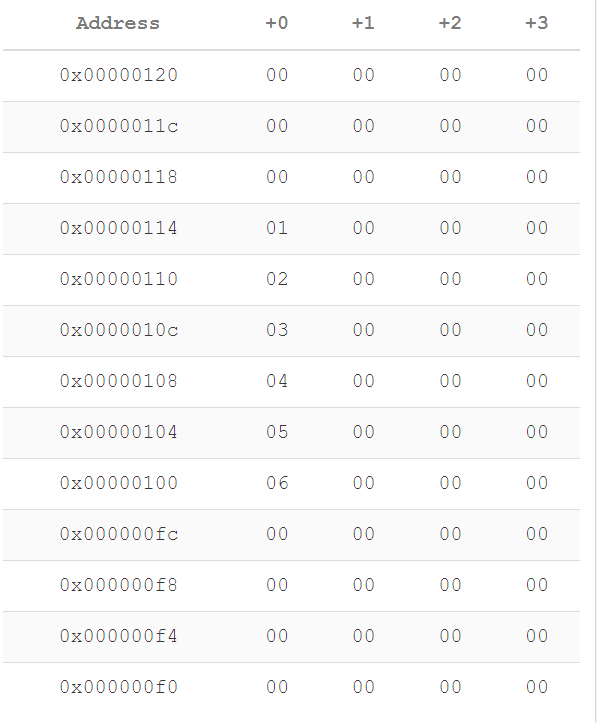
\includegraphics[width=0.8\textwidth]{before.png}
    \caption{Image of Memory before Sorting}
    \label{fig:SelectionSort}
\end{figure}

\begin{figure}[h]
    \centering
    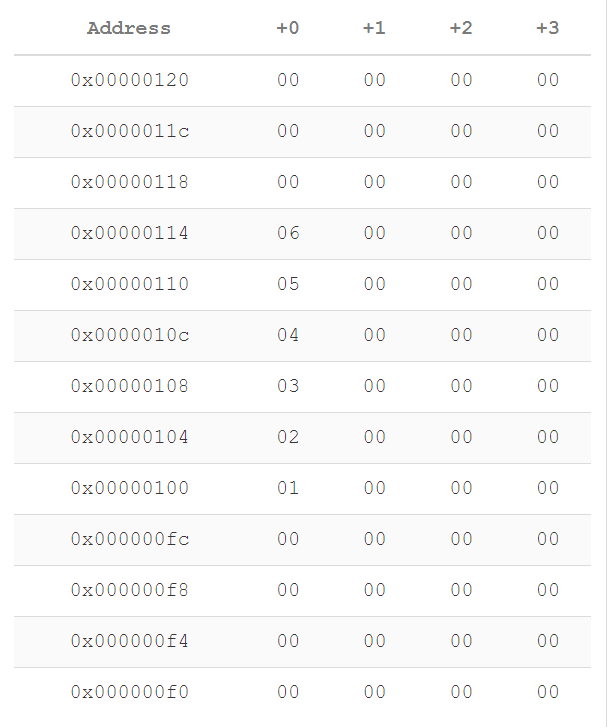
\includegraphics[width=0.8\textwidth]{after.png}
    \caption{Image of Memory after Sorting}
    \label{fig:SelectionSort2}
\end{figure}

\section{Design Modules}

\subsection{RISC-V Processor}

\begin{lstlisting}[caption={RISC-V Design Module Code}, captionpos=b, language=RISC-V]
`timescale 1ns / 1ps

module risc5processor(
    input clk,
    input reset,
    output wire [63:0] PC_In,
    output wire [63:0] PC_Out, // Instruction address
    output wire [31:0] instruction,
    output wire [4:0] rs1, 
    output wire [4:0] rs2, 
    output wire [4:0] rd,
    output wire [63:0] WriteData,
    output wire [63:0] readData1,
    output wire [63:0] readData2,
    output wire [63:0] imm_data,
    output wire [63:0] Result,
    output wire ZERO,
    output wire [63:0] Read_Data,
    output wire [6:0] opcode,
    output wire [2:0] funct3,
    output wire [6:0] funct7,
    output wire Branch,
    output wire MemRead,
    output wire MemtoReg,
    output wire MemWrite,
    output wire ALUSrc,
    output wire Regwrite,
    output wire [63:0] ele1,
    output wire [63:0] ele2,
    output wire [63:0] ele3,
    output wire [63:0] ele4,
    output wire [63:0] ele5,
    output wire [63:0] ele6
    );

    wire [63:0] out1;
    wire [63:0] out2;
    wire [1:0] ALUOp;
    wire [3:0] Operation;
    wire [63:0] data_out;
    
    //The code below is for program counter to go to next address
    Program_Counter pc (clk,reset, PC_In, PC_Out);
    
    //Add +4 to previous instruction for next instruction
    Adder add1 (PC_Out, 64`d4, out1);
    
    //Code below is for instruction memory instantiation
    Instruction_Memory insmem (PC_Out, instruction);
    
    //Code below is for instruction parser instantiation
    InsParser inspar (instruction, opcode, rd, funct3, rs1, rs2, funct7);
    
    //Code below is for control unit instantiation
    Control_Unit conunit (opcode, Branch, MemRead, MemtoReg, MemWrite, ALUSrc, Regwrite, ALUOp);
    
    //Code below is for register file instantiation
    registerFile regf (WriteData, rs1, rs2,rd, Regwrite, clk, reset, readData1, readData2); 
    
    //Code below is for immediate generator instantiation
    ImmGen immgen (instruction, imm_data);
    
    //Code below is for alu control instantiation
    ALU_Control ALUcont (ALUOp, {instruction[30], instruction[14:12]}, Operation);
    
    //Code below is for ALU mux instantiation to choose imm data/readdata2
    Mux ALUs (readData2, imm_data, ALUSrc, data_out); 
    
    //Code below is for ALU instantiation    
    ALU_64_bit ALU (readData1, data_out, Operation, Result, ZERO);
    
    //Code below is for data memory instantiation
    Data_Memory datamem (Result, readData2, clk, MemWrite, MemRead, Read_Data, ele1, ele2, ele3, ele4, ele5, ele6);
    
    //Code below is for data memory mux instantiation to select between alu result or read data for R-type/S-type/I-type ins   
    Mux memreg (Result, Read_Data, MemtoReg, WriteData); 
    
    //Code below is for branch adder instantiation to add branch and prev instruction address.
    Adder add2 (PC_Out,(imm_data << 1),out2);
    
    //code below is for program counter mux instantiation to select between adder +4 instruction or branch ins
    Mux PCs (out1, out2, (Branch & ZERO) , PC_In); 
    
endmodule  
\end{lstlisting}

\section{Simulation Sources}

\begin{lstlisting}[caption={RISC-V Simulation Source Code}, captionpos=b, language=RISC-V]
`timescale 1ns / 1ps

module risc5tb();
    reg clk;
    reg reset;
    wire [63:0] PC_In;
    wire [63:0] PC_Out;
    wire [31:0] instruction;
    wire [4:0] rs1; 
    wire [4:0] rs2; 
    wire [4:0] rd;
    wire [63:0] WriteData;
    wire [63:0] readData1;
    wire [63:0] readData2;
    wire [63:0] imm_data;
    wire [63:0] Result;
    wire ZERO;
    wire [63:0] Read_Data;
    wire [6:0] opcode;
    wire [2:0] funct3;
    wire [6:0] funct7;
    wire [63:0] ele1;
    wire [63:0] ele2;
    wire [63:0] ele3;
    wire [63:0] ele4;
    wire [63:0] ele5;
    wire [63:0] ele6;
    wire Branch;
    wire MemRead;
    wire MemtoReg;
    wire MemWrite;
    wire ALUSrc;
    wire Regwrite;
    
    //Instantiating RISC V processor 
    risc5processor processor (clk, reset, PC_In, PC_Out, instruction, rs1, rs2, rd, WriteData, readData1, readData2, imm_data, Result, ZERO, Read_Data, opcode, funct3, funct7, Branch, MemRead, MemtoReg, MemWrite, ALUSrc, Regwrite, ele1, ele2, ele3, ele4, ele5, ele6);

        initial
            begin
            clk = 1'b0;
            reset = 1'b1;
                #10
            reset = 1'b0;
            end
            
            always
            begin
                #5
                clk = ~clk;
            end 
        
endmodule

\end{lstlisting}

\end{document}
